\chapter{时间,空间和运动学}\label{chp:01}

\section[时间]{\makebox[5em][s]{时间}}\label{sec:01.01}

描写物体的运动,要用时间和空间这两个概念。因此,我们
先来对时间、空间本身作一些分析。

时间和空间可以说是最平凡的概念了,因为在日常生活中也
常常用到它们。不过,若问什么是时间?什么是空间?却又不容易
找到恰当的答案。其实,这是两个很难的问题。尽管有不少关于
时间和空间的定义,但大都不能令人满意。一种或许可以接受的
说法是:时间、空间是物理事件之间的一种次序,时间用以表述
事物之同的顺序,空间用以表述事件相互之间的位形。

没有满意的“严格”的理论定义,并不妨碍时间和空间二者
在物理中的使用。因为,物理学是一门基于实验的科学,在考查
物理学的概念或物理量的时候,首先应当注意它与实验之间是否
有明确的、不含糊的关系。对于时间和空间这两个基本概念来说,
首要的问题似不是去追究它们的“纯粹”定义,而是应当了解它
们是怎样量度的。

量度时间,通常是用钟和表。然而,钟和表并不是测量时间
的唯一的工具。原则上。任何具有重复性的过程或现象,都可以
作为测量时间的一种钟。自然界里有许多重复性的过程,其中有
一些我们早已把它们当作计时标准了。例如,太阳的升没表示天;
四季的循环称作年;月亮的盈亏是农历的月。其他的循环过程,
如双星的旋转、人体的脉搏、吊灯的摆动,分子的振动等等,也
都可以用作测时的工具。

更一般地说,只要知道了某个物理现象随时间的变化,尽管
它不是重复性的过程,也可以用来测定时间。譬如,我们能从一
个人的容貌估计出他的年龄,因为容貌这个量与时间之间有确定
的关系。这个例子虽然很普通,但某些有用的测时方法与此是很
相似的。在确定星体的年龄时,常常就是根据星体的颜色。

钟的种类很多,但有好有坏。比较两个人的脉搏,就会发现
它们之间经常有明显的快慢波动,所以,人的脉搏不是一种好钟,
它不够稳定。如果比较一下两个单摆的周期,就会发现它们稳定
多了。地球自转则是更稳定的钟。
\begin{figure}[!h]
  \centering
  \includegraphics[height=8cm]{figure/fig01.01}
  \caption{不同年代的时间测量精度}\label{fig:01.01}
\end{figure}

\clearpage
图\ref{fig:01.01}给出不同年代用不同的钟测量时间所达到的精度。可以
看到,地球自转要比各种机械的钟都好。所以,1967年以前是用
地球自转作为标准钟。原子钟是比地球自转更加稳定的钟,现代
的精密计时都是用原子钟了。

\begin{table}[!h]
  \centering
  \caption{一些典型物理现象的时间尺度}\label{tab:01.01}
  \begin{tabular}{c}
    \toprule
    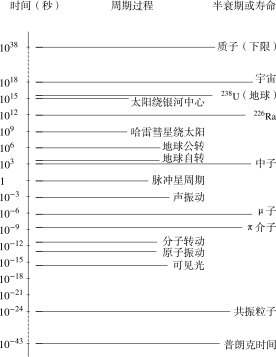
\includegraphics[width=0.8\linewidth]{figure/tab01.01} \\
    \bottomrule
  \end{tabular}
\end{table}
\clearpage
1967年10月在第十三届国际度量衡会议上通过了新的标准
钟,它对一秒的时间作如下的规定;位于海平面上的$^{133}$Cs原子
的基态的两个超精细能级在零磁场中跃迁辐射的周期$T$与$ 1 $秒的
关系为
\begin{equation*}
  1 \,\text{秒} = 9,192,631,770\,T
\end{equation*}

表\ref{tab:01.01}~列举了一些典型现象的时间尺度。目前,物理学中涉及
的最长的时间是:\num{e38}秒,它是质子寿命的下限。宇宙的年龄大约
是 \num{6e17}秒,即$ 200 $亿年。牛顿力学所涉及的时间尺度大约是
\num{e-3}$\sim$\num{e15}秒,即从声振动的周期到太阳绕银河中心转动的周期。
粒子物理的时间尺度都很小。$\mu$子的寿命是 \num{2e-6} 秒。已经算是
极长寿的了。最短寿的是一些共振粒子,它们的寿命只约有 \num{e-24}
秒。目前物理学中涉及的最小的时间是 \num{e-42}秒,称为普朗克时
间。普朗克时间被认为是最小的时间,比普朗克时间还要小的范
围内,时间的概念可能就不再适用了。

\documentclass[../outline-of-mechanics.tex]{subfiles}

\begin{document}

\section{芝诺佯谬和时间的度量}\label{sec:01.02}

古希腊哲学家芝诺有一个很著名的论证:跑得最快的神话英
雄阿基里斯是永远追不上跑得最慢的东西 (例如一只龟) 的。他的
论证如下:因为开始时阿基里斯是在龟的后面,所以,阿基里斯
要追上龟,他必定先要到达龟的出发点,这要用有限的时间,在
这段时间里龟必定向前跑了,到达前面的一点,而当阿基里斯再
到达这点时,龟必定又已到达更前面的一点。如此重复下去,就
是进行无穷多次,龟也总不会落在阿基里斯之后。

这个论证被称为芝诺佯谬,如何解开这个佯谬?

关键是在芝诺佯谬中用了两种不同的时间度量。按上节的讨
论,任何一种具有重复性的过程。都可以做为“钟”,用其重复
的次数来量度时间。芝诺问题中。除了“普通”钟所测得的时间
$t$,还利用了一种很特别的钟,该钟使用的重复性过程是:阿基里
斯逐次地到达龟在前一次的出发点。我们称这种钟叫芝诺钟,它
测得的时间为$t'$。

\begin{figure}[!h]
  \centering
  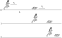
\includegraphics{figure/fig01.02}
  \caption{芝诺时的定义}\label{fig:01.02}
\end{figure}

如图\ref{fig:01.02},阿基里斯和龟在开始时相距为$L$,速度分别为$v_1$及
$v_2$,并且$v_1>v_2$。如果用普通的钟,则阿基里斯将在
\begin{equation}
  t=L/\left(v_1-v_2\right)
  \label{eqn:01.02.01}
\end{equation}
时,赶上龟;当$t>L/\left(v_1-v_2\right)$时,阿基里斯就超过龟了。

图中左边的数字表示的是芝诺时$t'$。当$t'=1$时,阿基里斯到
达龟在0时的出发点;当$t'=2$时,阿基里斯到达龟在1时的出发
点。一般地,当$t'=n$时,阿基里斯到达龟在$t'=n-1$时的位置。
显然,只有当$t'\to\infty$时,阿基里斯才能逼近龟,对于任何有限的
$t'$,阿基里斯总是落在龟的后面。这就是芝诺的结论。

因此,芝诺断言:“阿基里斯永远也追不上龟。”这里“永
远”的含意是$t'\to\infty$。,即芝诺时间的无限。

现在我们来讨论普通时$t$与芝诺时$t'$之间的变换关系。不难
验证表\ref{tab:01.02} 给出的两种时间的对应。因此,一般有
{\setlength{\mathindent}{4em}
\begin{equation}\label{eqn:01.02.02}
  t=\sum_{n=0}^{t^{\prime}-1} \frac{L}{v_{1}}{\left(\frac{v_{2}}{v_{1}}\right)}^{n}=\frac{L}{v_{1}-v_{2}}\left[1-{\left(\frac{v_{2}}{v_{1}}\right)}^{t'}\right]
\end{equation}}%
或者
\begin{equation}
  t^{\prime}=\frac{1}{\ln \left(v_{2} / v_{1}\right)} \ln \left[1-\left(\frac{v_{1}-v_{2}}{L}\right) t\right]
  \label{eqn:01.02.03}
\end{equation}%
式\eqref{eqn:01.02.02}或式\eqref{eqn:01.02.03}称为芝诺变换。它给出的$t'$与$t$的关系。在
图\ref{fig:01.03}~中画出。

\begin{table}[!h]
  %\renewcommand\arraystretch{1.6}
  \centering
  \caption{普通时与芝诺时的关系}\label{tab:01.02}
  \zihao{-5}
  \begin{tblr}{colsep=2em,row{2-Z}={rowsep=0em},colspec={c|X}}
    \toprule
    芝诺时($t'$) & \SetCell{c}普通时($t$)                                                                                                        \\
    \midrule
    0         & 0                                                                                                                          \\[1.75ex]
    1         & $\dfrac{L}{v_1}$                                                                                                           \\[1.75ex]
    2         & $\dfrac{L}{v_1} +\dfrac{L}{v_1}\cdot\dfrac{v_2}{v_1}$                                                                      \\[1.75ex]
    \vdots    & \vdots                                                                                                                     \\
    $n$       & $\dfrac{L}{v_1} + \dfrac{L}{v_1}\cdot\dfrac{v_2}{v_1} + \cdots +\dfrac{L}{v_1}\cdot{\left(\dfrac{v_2}{v_1}\right)}^{n-1} $ \\[1.75ex]
              & $= \displaystyle \sum_{i=0}^{n-1} \frac{L}{v_1}{\left(\frac{v_2}{v_1}\right)}^i$                                           \\
    \bottomrule
  \end{tblr}
  \vspace{-0.8em}
\end{table}

由图\ref{fig:01.03}看到,芝诺变换是有奇性的,即当$t=L/\left(v_1-v_2\right)$时,
$t'\rightarrow\infty$。所以,当芝诺时$t'$从零变化到无限时,它只覆盖了普通时
$t$上的一个有限范围,即从零到$ L/\left(v_1-v_2\right) $。

因此,芝诺佯谬之“佯”,是由于芝诺把\CJKunderdot{永远}理解为$t'\rightarrow\infty$。
他认为$t'\rightarrow\infty$之后就没有时间了,故$t'\rightarrow\infty$相当于永远。实际上,
从图\ref{fig:01.03} 看到,在芝诺时$ t' $到达无限之后。还是有时间的。但是,
在该范围,即$ t>L/\left(v_1-v_2\right) $,用芝诺钟已经无法度量它们了。简
言之,芝诺的佯谬,来源于芝诺时的局限性,芝诺时不可能度量
阿基里斯追上龟之后的现象。

芝诺佯谬给我们的启示是,时间与时间的度量不同,一种时

\begin{wrapfigure}[10]{10}{48mm}
  %\vspace{-0.5em}
  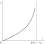
\includegraphics{figure/fig01.03}
  \caption{芝诺时的定义}\label{fig:01.03}
  %\vspace{-1.2em}
\end{wrapfigure}
\noindent 间的度量达到无限之后,还是可以有时间的;反之,一种时
间的度量达到无限,从其他的度量看,可能是有限的。

芝诺佯谬还启发我们提出一个更深入的问题,即所谓普通钟
或日常钟是否也具有芝诺钟那种局限性?当日常钟$t$的读数达到
无限之后,是否也还有时间?是否有$t$也无法度量的现象,即在
$t\rightarrow\infty$之外的现象?现代物理学的研究,对这些
问题的回答都是肯定的。

\end{document}

\section[长度]{\makebox[5em][s]{长度}}\label{sec:01.03}

长度是空间的一个基本性质。

对长度的测量,在日常的范围中,是用各种各样的尺,如米
尺、千分尺、螺旋测微计等等。对于不能用尺直接加以测量的小
尺度,可以求助于光学方法。在精密机床上常有光学测量装置;
测定胰岛索中原子的位置,是用X衍射方法。对于大的尺度,
也不能直接用尺去测量,也要求助于光。测量月亮与地球的距离
可以用激光测距的方法;测量一些不太远的恒星,可以用三角学
方法,利用恒星发出的光。至于银河系之外的遥远天体的距离,
同样是用它们发光的一些特征来测定的。

最近,长度的单位和标准,也用光来规定了。

长度的位单是米。1960年以前,用铂铱米尺作为标准尺,规
定米的大小。1960年以后,改用光的波长作为标准。在第十一届
国际计量大会上,正式通过的“米”的定义是l米等于$^{86}$Kr原子
\clearpage\noindent
的$2\rm{p}_{10}$和$5\rm{d}_5$
能级之间跃迁时所对应的辐射在真空中的波长$\lambda$的1,650,763.73倍,即
\begin{equation*}
 1 \text{米} = 1,650,763.73 \, \lambda
\end{equation*}

1983年10月召开的第十七届国际计量大会上已正式通过了
\begin{table}[!h]
 \centering
 \caption{一些典型物理现象的空间尺度}
 \label{tab:01.03}
 \begin{tabular*}{\linewidth}{>{\centering}m{\linewidth}c}
 \toprule
 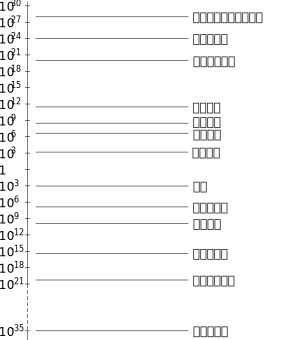
\includegraphics[width=0.8\linewidth]{figure/tab01.03} & \\
 \bottomrule
 \end{tabular*}
\end{table}
\clearpage

\noindent 新的米的定义,即用光速值来定义“米”,以代替1960年的规定。
新的米的定义是,米是光在真空中在$ 1/299,792,458 $秒的时间间隔
内所传播的路程长度。按这种新的定义,光速$ c $是一固定的常数,即
\begin{equation*}
 c = 299,792,458 \, \text{米/秒}
\end{equation*}

表\ref{tab:01.03}中列举了一些典型现象的空间尺度。目前,物理学中涉
及的最太长度是$10^{28}$米,它是宇宙曲率半径的下限;已达到的最
小长度为$10^{-20}$米,它是弱电统一的特征尺度。普朗克长度约为
$10^{-35}$米,被认为是最小的长度,意思是说,在比普朗克长度更小
的范围内,长度的概念可能就不再适用了。

\section[参考系]{\makebox[5em][s]{参考系}}\label{sec:01.04}

牛顿力学所研究的对象是物体的机械运动。从我们日常见到
的车行马跑,及至大到月亮、太阳等星体的运行,小到分子、原子、
粒子的一些飞行,都是属于这一类运动。这类运动的共同特点,
就是物体在空间的位置时刻在变化着。当然,静止的状态、平衡
的状态也是力学的内容之一。

牛顿意义下的运动学,就是研究如何描写物体位置的变化。

研究问题总是从简单的情况入手。我们首先讨论一种被称为
质点的物体,即大小为零的物体。我们知道,任何具体的物体总
是有一定大小的,没有任何一个物体与质点完全等价。但是,对
于某些特定的运动来说,可以足够准确地把物体看作一个质点。
譬如,在讨论地球绕太阳的公转时,由于地球的半径(约$ 6,400 $公
里)比地球与太阳的距离(约$ 149,504,000 $公里)小得多,把地球作
为质点是相当好的近似,或者说,在此情况下,将地球作为质点
处理,是一个足够准确的模型。显然,这种模型是有一定适用限
度的。当讨论到地表问题时,再把地球看作质点就大谬不然了。

质点是一个物理对象。对于一个物理对象,用什么数学语言
来描写,这并不是一件很自然的事情,我们知道,任何一种数学
只是一种逻辑体系,一种逻辑体系能不能正确地描写我们的物理
对象,是要认真研究的。物理上,就是要寻找那种能正确地描写
物理对象的数学。在牛顿力学中,质点的空间几何性质,相当于
欧几里德几何上的点。在解析几何中,点的位置是由它的坐标值
来确定的。质点的位置也可以用这种坐标方法来给定。利用坐标
方法,首先要给出坐标系,坐标值总是相对于一定的坐标系而言
的。在数学上,坐标系的选取是完全任意的,但在物理上,我们
要对描写运动的各种物理量进行实际测量,坐标必须固定在一定
\begin{wrapfigure}[11]{l}{13em}
  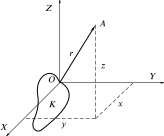
\includegraphics{figure/fig01.04}
  \caption{参考系$K$及参考坐标系$OXYZ$}
  \label{fig:01.04}
\end{wrapfigure}
的物体上。例如,如果选取物体$K$上的某点$O$为坐标原点,并选
定$x$,$y$,$z$三个轴,质点$A$的位置即由$x$,$y$,$z$所确定(图\ref{fig:01.04})。
这时,我们称所选取的物体$K$为参考系,而称坐标系$OXYZ$为参
考坐标系。

除了坐标方法外,也可以利用矢量方法来描写质点A的位
置。我们定义质点$A$的位置矢量$\vec{r}$的大小为$OA$的长度,而方向从
$O$指向$A$。用这个矢量就完全确定了质点$A$的位置。在图1.4的坐
标系中,位置矢量$r$的分量就是坐标$x$,$y$,$z$,或写为
\begin{equation}\label{eqn:01.04.01}
  \vec{r}=x\vec{i}+y\vec{j}+z\vec{k}
\end{equation}
其中$\vec{i}$,$\vec{j}$,$\vec{k}$分别为$X$,$Y$,$Z$轴上的单位矢量,上述两种描述
质点$A$的位置的方法,是完全等价的。

参考系的选择是任意的,可以不用参考系$K$,而用另外一
\begin{wrapfigure}[9]{r}{13.2em}
  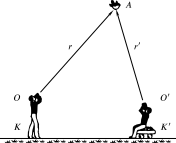
\includegraphics{figure/fig01.05}
  \caption{从不同参考系观察同一运动}
  \label{fig:01.05}
\end{wrapfigure}
个参考系$K'$,譬如,用运动着的车辆来描述质点$A$的位置。由图\ref{fig:01.05}
看到,对干参考系$K$,质点$A$的位置由矢量$\vec{r}$描写,而对于参考
系$K'$,由$\vec{r'}$描写。可见,对于同一个质点的位置,用不同参考系
来描写时,具有不同的位置矢量。就这一点,我们可以说,位
置是具有相对性的物理量。涉及物理量的相对性与绝对性的问题,
以后我们还要专门论述。

\section[轨迹]{\makebox[5em][s]{轨迹}}\label{sec:01.05}

谁都看到过,当喷气式飞机在飞行的时候,它的尾部泄出的
白烟在天空中构成形状美丽的各样曲线。这些曲线反映了飞机所
行经的路程。质点在运动中所经过的各点在空间连成一条曲线,
这条曲线我们称之为轨迹。

\begin{figure}[!h]
  \hspace{3em}
  \subfigure[\null]{
    \label{fig:01.06a}
    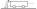
\includegraphics{figure/fig01.06a}
  }
  \hspace{3em}
  \subfigure[\null]{
    \label{fig:01.06b}
    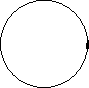
\includegraphics{figure/fig01.06b}
  }

  \hspace{3.7em}
  \subfigure[\null]{
    \label{fig:01.06c}
    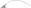
\includegraphics{figure/fig01.06c}
  }
  \hspace{1.3em}
  \subfigure[\null]{
    \label{fig:01.06d}
    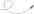
\includegraphics{figure/fig01.06d}
  }
  \caption{各种运动的轨迹}
  \label{fig:01.06}
\end{figure}

\clearpage

从图\ref{fig:01.06}看到,各种运动的轨迹形状是不同的;\subref{fig:01.06a}图是直线,
\subref{fig:01.06b}图是圆周,\subref{fig:01.06c}图是抛物线,\subref{fig:01.06d}图是一般曲线。依照轨迹形状
的不同,可以把运动分为直线运动和曲线运动两大类。

如何描写轨迹呢?可利用曲线方程来描写。譬如,曲线方程 \begin{equation*}
  \begin{aligned}
     & x^2+y^2=r^2 \\
     & z=0
  \end{aligned}
\end{equation*}
就描写了在$z=0$平面上半径为$r$的圆周运动的轨迹。一般曲线方
程可以表示成
\begin{equation*}
  \begin{aligned}
    f_1\left(x,y,z\right)=0 \\
    f_2\left(x,y,z\right)=0
  \end{aligned}
\end{equation*}

在历史上很长一个时期内,人们只注重轨迹形状的研究,例
如行星走圆形,落体走直线。我们知道,质点运动是位置的变化,
它涉及空间和时间两方面。轨迹形状只反映了运动的空间方面的
性质,它对于研究运动还是不够的,因为轨迹还没有把质点运动
的情况全部表述出来,特别是没有表述它的动态性质。百米赛跑
时,所有运动员的轨迹都是直线,但他们各自的运动情况并不全
同,否则就分不出名次了。我们不仅应该知道轨迹,而且还应知
道质点经过轨迹上各点的时刻。运动是在时间、空间里的现象,
关键是把时间描写和空间描写联系起来。直到牛顿之前不久,才
特别强调了这一点。

下面,我们举两个直线运动的例子。

对于在平直铁轨上稳定运动的列车上的某一点,所测得的各
时刻的位置列于表\ref{tab:01.04}中,其中位置坐标$x$是以铁轨为参考系的(图\ref{fig:01.07})。
\begin{table}[h]
  \caption{}
  \label{tab:01.04}
  \centering
  \zihao{-5}
  \begin{tblr}{c*{6}{|X[c]}}
    \toprule
    时\hspace{2em}间(秒) & 0 & 1  & 2  & 3  & 4  & 5  \\
    \midrule
    位置坐标(米)           & 0 & 17 & 34 & 51 & 68 & 85 \\
    \bottomrule
  \end{tblr}
\end{table}

\begin{figure}[!h]
  \centering
  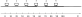
\includegraphics{figure/fig01.07}
  \caption{列车的运动}
  \label{fig:01.07}
\end{figure}

对于从地面上某一高度自由落下的质点(称为自由落体),轨
迹也是一条直线。如果我们取如图\ref{fig:01.08}所示的坐标系,则所测得的
质点在各时刻的位置列在表\ref{tab:01.05}中。
\begin{table}[!h]
  \caption{}
  \label{tab:01.05}
  \zihao{-5}
  \centering
  \begin{tblr}{c*{5}{|X[c]}}
    \toprule
    时\hspace{2em}间(秒) & 0 & 1   & 2    & 3    & 4    \\
    \midrule
    位置坐标(米)           & 0 & 4.9 & 19.6 & 44.1 & 78.4 \\
    \bottomrule
  \end{tblr}
\end{table}

用数学的语言说,表\ref{tab:01.04}~和表\ref{tab:01.05}~是给出了质点的位置坐标与
时间之间的函数关系,这个函数关系$x\left(t\right)$,称之为轨迹函数,或
\begin{wrapfigure}[14]{l}{8em}
  \centering
  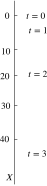
\includegraphics{figure/fig01.08}
  \\ ~ \\
  \caption{落体的运动}
  \label{fig:01.08}
\end{wrapfigure}
运动方程式、运动解。

为了便于进行计算,我们常希望能把轨迹
函数$x\left(t\right)$写成简单的分析表达式。对于表\ref{tab:01.04}~
的$x\left(t\right)$,可以写成
\begin{equation}\label{eqn:01.05.01}
  x=17t
\end{equation}
对于表\ref{tab:01.05}~的运动,可以写成$x=4.9t^2$。

对于曲线运动,轨迹函数就是位置矢量$\vec{r}$作为时间
$t$的函数,亦即$\vec{r}\left(t\right)$。随着$t$的变化,位置矢量$\vec{r}$的
端点在空间所划出的曲线,就是质点运动的轨迹(图\ref{fig:01.09})。也可
以用质点的三个坐标的函数$x\left(t\right)$,$y\left(t\right)$及$z\left(t\right)$来描写运
动,它们与$\vec{r}\left(t\right)$的关系是
\clearpage
\begin{equation}\label{eqn:01.05.02}
  \vec{r}\left(t\right)=x\left(t\right)\vec{i}+y\left(t\right)\vec{j}+z\left(t\right)\vec{k}
\end{equation}

\begin{wrapfigure}[7]{r}{11em}
  \centering
  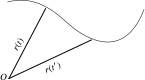
\includegraphics{figure/fig01.09}
  \caption{曲线运动}
  \label{fig:01.09}
\end{wrapfigure}
轨迹也具有相对性。譬如对于从地面上某一高度自由下落的质点,以
地面为参考系,看到轨迹是一条直线;而相对于沿平直铁轨稳定运行的
列车来说,轨迹则是一条抛物线。同一个物体的运动,在不同的参考系中
看到的轨迹形状不一定相同。

另一方面,对于时间,也必须选取一定的标准,即选取时间
原点,才能进行测量。而时间原点的选取,也有任意性,不同的
选取法,使轨迹函数的形式也有些差别。

因此,参考系的概念要作些扩充。选取一个参考系应包括:
给定放置在某物体上的坐标系,作为测量空间的标准;以及给定
一个钟,作为测量时间的标准。

\section{速度的瞬时性}\label{sec:01.06}

机械运动的现象,给了我们对“快”、“慢”的经验认识。
火车比轮船快,飞机比火车快,而火箭更比飞机快等等。反映质
点运动快慢的物理量就是速度,或者确切地说,是速度的数值大小。

先以直线运动为例,当时刻$ t_1 $时,质点$ A $的位置坐标为$ x\left(t_1\right) $,
当$ t_2 $时,它的坐标为$ x\left(t_2\right) $,我们就用下式来定义质点$ A $在$ t_1 $到
$ t_2 $时间间隔内的平均速度:
\begin{equation}
 \langle v\rangle_{t_{1} \rightarrow t_{2}}=\frac{x\left(t_{2}\right)-x\left(t_{1}\right)}{t_{2}-t_{1}} \label{eqn:01.06.01}
\end{equation}
符号$\langle ~ \rangle$表示所讨论的量的平均值。$\langle v\rangle_{t_{1} \rightarrow t_{2}}$的数值表示质点
在时
\clearpage
\noindent 间间隔$t_{1} \rightarrow t_{2}$中每单位时同平均走过的距离,它的单位是
米/秒。利用表\ref{tab:01.04}所给出的运动进行计算,就有:在第1秒末到
第2秒末间隔中,
\begin{equation*}
 \langle v\rangle_{1 \rightarrow 2}=\frac{34-17}{2-1}=17\,\text{米/秒}
\end{equation*}
在第3秒末到第5秒末间隔中,
\begin{equation*}
 \langle v\rangle_{3 \rightarrow 5}=\frac{85-51}{5-3}=17\,\text{米/秒}
\end{equation*}
选两个时间间隔中平均速度是一样的。事实上,如果利用分析表
达式\eqref{eqn:01.05.01}~来计算,就会发现对任何时间间隔,运动的平均速度
都是17米/秒。这种对于任何时间间隔平均速度总不变的运动,称
为匀速直线运动。

由表\ref{tab:01.05}~或$x=4.9t^2$所示的自由落体运动,情况就不同了:
在第1秒末到第3秒束的问隔中,
\begin{equation*}
 \langle v\rangle_{1 \rightarrow 3}=\frac{44.1-4.9}{3-1}=19.6\,\text{米/秒}
\end{equation*}
在第1秒末到第2秒末的间隔中,
\begin{equation*}
 \langle v\rangle_{1 \rightarrow 2}=\frac{19.6-4.9}{2-1}=14.7\,\text{米/秒}
\end{equation*}
在第2秒末到第3秒末的间隔中,
\begin{equation*}
 \langle v\rangle_{2 \rightarrow 3}=\frac{44.1-19.6}{3-2}=25.4\,\text{米/秒}
\end{equation*}
对于不同的时间间隔。自由落体的平均速度不相同。这种运动称
为变速运动。从上面所给出的三个平均速度可知,自由落体在第
1秒末到第3秒末的两秒钟时间间隔中并非匀速,它在前一秒钟
(即第1秒末到第2秒末)平均速度较小,在后一秒钟(即第2秒末
到第3秒末)平均速度较大。从这一点上可以充分反映出平均速度
往往不足以描写变速运动的细致情况。这是平均速度概
念的弱点。求平均速度的时间间隔取得越大,它对快慢的描述就越粗略;
反之,时间间隔越小,对快慢的描述也就越精确。在上例中,虽
然取1秒的时间间隔,比取2秒的时间间隔要好一些,但是在一
秒钟的时间间隔内,自由落体仍然不是匀速的。这种情况迫使我
们把计算平均速度的时间间隔取得尽可能地小。

为了便于进一步讨论,我们将式\ref{eqn:01.06.01}~中的
$t_2$表示成$t_2=t_1+\Delta t$,这个$\Delta t$就是求平均速
度所选用的时间间隔。现在来求从第1秒末到第$1+\Delta t$秒末
的间隔中,自由落体的平均速度。利用$x=4.9t^2$得到
\begin{equation*}
 \begin{aligned}
 \langle v\rangle_{1 \rightarrow 1+\Delta t} & =\frac{x\left(1+\Delta t\right)-x\left(1\right)}{1+\Delta t-1} \\
 & =\frac{4.9 \times\left(1+\Delta t\right)^{2}-4.9 \times 1^{2}}{\Delta t} \\
 & =\left(9.8+4.9 \Delta t\right) \text { 米/秒 }
 \end{aligned}
\end{equation*}
此式再次表明,从第1秒末开始取不同的时间间隔$\Delta t$,所得的平
均速度是不相同的。既然$\Delta t$越小描述得越精确,我们取
$\Delta t$为无限小,或者相当于$\Delta t \rightarrow 0$的
极限情况,这时平均速度变成为:
\begin{equation*}
 \lim _{\Delta t \rightarrow 0}\left(9.8+4.9 \Delta t\right)=9.8 \text { 米/秒 }
\end{equation*}
这个9.8米/秒的物理意义是自由落体在第1秒末的一个无限小时
间间隔中的平均速度,我们称这个值为自由落体在第1秒末的瞬
时速度。瞬时速度与平均速度这两个概念的重要区别在于:平均
速度总是与一段有限的时间间隔相联系,它是描述一段运动过程
的物理量;相反,瞬时速度与一个时刻相联系,它是描述运动的
瞬时性质的物理量。有了瞬时速度这个概念,使我们对运动的认
识大为深化。

用类似的手续不难求出自由落体运动在任何时刻t的瞬时速
度$v\left(t\right)$,只要将上述的1及$1+\Delta t$分别代之以$t$及$t+\Delta t$,并取
于$\Delta t \rightarrow 0$的极限值就可以了。故有

\begin{equation}\label{eqn:01.06.02}
 \begin{aligned}
 v\left(t\right) & =\lim _{\Delta t \rightarrow 0} \frac{x\left(t+\Delta t\right)-x\left(t\right)}{\Delta t} \\
 & =\lim _{\Delta t \rightarrow 0} \frac{4.9 \times\left(t+\Delta t\right)^{2}-4.9 \times t^{2}}{\Delta t} \\
 & =\lim _{\Delta t \rightarrow 0}\left(9.8 t+4.9 \Delta t\right) \\
 & =9.8 t
 \end{aligned}
\end{equation}
此式给出了自由落体在每个时刻的瞬时速度。根据这个结果,我
们再强调一遍,自由落体的运动快慢是时刻变化着的。你用平均
速度来描写它,无论$\Delta t$取如何小的有限值,即使小到$\Delta t$=0.001
秒,依然不够精确,因为在这0.001秒中质点依然不是匀速运动
的。只有$\Delta t$趋于无限小,给出了每个时刻$t$的瞬时速度,了解了
质点运动在每一瞬时的快慢,才算最精确地反映了质点运动的快
慢。

对于任何直线运动,它的瞬时速度都可以用类似方式来确
定:
\begin{equation*}
 v\left(t\right)=\lim _{\Delta t \rightarrow 0} \frac{x\left(t+\Delta t\right)-x\left(t\right)}{\Delta t}
\end{equation*}
根据微积分学的知识,该极限就是轨迹函数$x\left(t\right)$对时间t的一阶
导数。即
\begin{equation}
 \begin{aligned}
 v\left(t\right) & =\lim _{\Delta t \rightarrow 0} \frac{x\left(t+\Delta t\right)-x\left(t\right)}{\Delta t} \\
 & =\lim _{\Delta t \rightarrow 0} \frac{\Delta x}{\Delta t}=\frac{\dif x}{\dif t} \label{eqn:01.06.03}
 \end{aligned}
\end{equation}
其中,$\Delta x=x\left(t+\Delta t\right)-x\left(t\right)$,是在$t\rightarrow t+\Delta t$时间间隔中质点位置
坐标的增量。以后我们提到的速度,一般都指瞬时速度。

我们看到,瞬时速度是利用数学上的微分概念来描写的。其
实,在历史上,正是由于牛顿在处理这类基本力学问题时需要一
种适当的数学工具,从而促使他创建了微积分学。这不仅使物理
概念得以准确地表述,而且也大大丰富了数学本身。这是牛顿的
巨大功绩之一。\ziju{-0.02}由此,我们再次看到,一个物理对象,用什么数学
语言描写并不是一件自然的事情,而是物理研究的一个核心课题。\ziju{0}

\begin{wrapfigure}[10]{r}{13em}
 \centering
 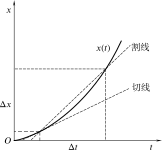
\includegraphics{figure/fig01.10}
 \caption{直线运动的$x \mathdash t$图}
 \label{fig:01.10}
\end{wrapfigure}
当质点作直线运动时,我们
可以设法求出它的位置时间曲线
(图\ref{fig:01.10})。从图中可以看出,平
均速度在数值上等于各段割线的
斜率,瞬时速度在数值上等于各
点的切线的斜率。所以在求出位
置时间曲线后,就可以从$x\left(t\right)$曲
线上求出各点的速度。

从平均速度的定义(\ref{eqn:01.06.01})式可以知道,$\langle v\rangle$可以有正值,
也可以有负值。当$x\left(t+\Delta t\right)<x\left(t\right)$时,$\langle v\rangle$为负。这种情况相当
于质点在$t$到$t+\Delta t$间隔中,总的说来是向负$x$方向运动的。所
以,$\langle v\rangle$的正负恰恰反映了运动的方向。通常称平均速度的绝对
值$|\langle v\rangle|$为平均速率。类似地,瞬时速度的绝对值$|\vec{v}\left(t\right)|$被称为
速率,而瞬时速度的正负,就表示质点在时刻$t$的运动方向。速
度$\vec{v}$不仅描述了运动的快慢,而且描述了运动方向。
\section{曲线运动的速度}\label{sec:01.07}

\ziju{-0.02}我们现在来推广上节关于直线运动的速度的概念。按图1.11,
质点作曲线运动,在时刻$t_1$,质点位置矢量为$\vec{r}\left(t_1\right)$,在时刻$t_2$,
位置矢量为$\vec{r}\left(t_2\right)$,则定义在$t_1$到$t_1$间隔中质点$ A $的平均速度为
\begin{equation}\label{eqn:01.07.01}
  \langle \vec{v} \rangle_{t_1\rightarrow t_2}=\frac{\vec{r}\left(t_2\right)-\vec{r}\left(t_1\right)}{t_2-t_1}=\frac{\Delta \vec{r}}{\Delta t}
\end{equation}

\clearpage\noindent 将其与式\eqref{eqn:01.06.01}~对比可见。只是将其中的$x\left(t\right)$换成了相应的
$\vec{r}\left(t\right)$。在\eqref{eqn:01.07.01}~中,$\Delta t=t_2-t_1$,$\Delta \vec{r}=\vec{r}\left(t_2\right)-\vec{r}\left(t_1\right)$,
后者是$t_1$到$t_2$间隔
\begin{wrapfigure}[8]{r}{12em}
  \centering
  \small
  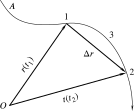
\includegraphics{figure/fig01.11}
  \caption{曲线运动的速度}
  \label{fig:01.11}
\end{wrapfigure}
中质点位置矢量的改变量,称为位移矢量。这个平均速度的定义表明,平均速度是矢量。根据矢量运算
规则,式\eqref{eqn:01.07.01}~所定义的$\langle \vec{v}\rangle_{t_1-t_2}$是在l到2的方向(图\ref{fig:01.11})。
另一方面,由图\ref{fig:01.11}~很清楚知道,在$t_1$到$t_2$时间内质点$A$的运
动方向并非总是沿着l到2的方向的,而是先从1向3方向运动,
然后从3向2方向运动,这些运动方向并不平行于1到2的方向。
所以平均速度所指的方向,只是质点$A$真实运动方向的平均。
也就是说,平均速度不但对于运动快慢的描写是粗
略的,而且对于运动方向的描写也是粗略的。

对式\eqref{eqn:01.07.01}~取$\Delta t \rightarrow 0$的极限,就得到瞬
时速度的定义。
\begin{equation}\label{eqn:01.07.02}
  \begin{aligned}
    \vec{v}\left(t\right) & =\lim _{\Delta t \rightarrow 0} \frac{\vec{r}\left(t+\Delta t\right)-\vec{r}\left(t\right)}{\Delta t} \\
                          & =\lim _{\Delta t \rightarrow 0} \frac{\Delta \vec{r}}{\Delta t} =\frac{\dif\vec{r}}{\dif t}
  \end{aligned}
\end{equation}
它是直线运动情况的式\eqref{eqn:01.06.03}的推广。如果利用式\eqref{eqn:01.04.01},则
有
\begin{equation}\label{eqn:01.07.03}
  \vec{v}\left(t\right)=\frac{\dif x\left(t\right)}{\dif t} \vec{i}+\frac{\dif y\left(t\right)}{\dif t} \vec{j}+\frac{\dif z\left(t\right)}{\dif t} \vec{k}
\end{equation}
所以三个坐标函数$x\left(t\right)$,$y\left(t\right)$,$z\left(t\right)$对时间t的导数分别是速度矢
量在三个坐标轴方向的分量:
\begin{equation}\label{eqn:01.07.04}
  v_{x}=\frac{\dif x\left(t\right)}{\dif t}, ~ v_{y}=\frac{\dif y\left(t\right)}{\dif t}, ~ v_{z}=\frac{\dif z\left(t\right)}{\dif t}
\end{equation}
\clearpage
\begin{wrapfigure}[7]{r}{13em}
  \centering
  \small
  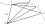
\includegraphics{figure/fig01.12}
  \caption{曲线运动的瞬时速度}
  \label{fig:01.12}
\end{wrapfigure}
由图\ref{fig:01.12},当$\Delta t$减小时,矢量$\vec{r}\left(t+\Delta t\right)$
逐渐向$\vec{r}\left(t\right)$靠拢,矢量$\Delta \vec{r}$相继从1,2变到1,3,
变到1,4……,在$\Delta t \rightarrow 0$的极限情况下,$\Delta \vec{r}$
的方向趋于轨迹曲线在点1的切线方向。这样,我们就得到一个
结论:瞬时速度$\vec{v}\left(t\right)$的方
向,就是轨迹曲线在相应点的切线方向。瞬时速度的大小$v$,按
定义\eqref{eqn:01.07.02}应为
\setlength{\mathindent}{15em}
\begin{equation*}
  \begin{aligned}
    v\equiv |\vec{v}| & =\left|\lim _{\Delta t \rightarrow 0} \frac{\Delta \vec{r}\left(t\right)}{\Delta t}\right| \\
                      & =\lim _{\Delta t \rightarrow 0} \frac{|\Delta \vec{r}|}{\Delta t}
  \end{aligned}
\end{equation*}

\setlength{\mathindent}{6em}
\begin{wrapfigure}[4]{l}{10em}
  \vspace{-6em}
  \centering
  \small
  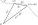
\includegraphics{figure/fig01.13}
  \caption{用路程长度$s\left(t\right)$来描写运动}
  \label{fig:01.13}
\end{wrapfigure}
\noindent 我们可以引入路程长度概念来描写运动。如图\ref{fig:01.13},若当$t=0$时,
质点在轨迹上的$P$处。则可定义函数$s\left(t\right)$,它表示质点到$t$时刻所
走过的路程的长度。显然,$\Delta s=s\left(t+\Delta t\right)-s\left(t\right)$表示
在$t$到$t+\Delta t$中质点所走过的路程的长度。一般$\Delta s$和
$|\Delta \vec{r}|$并不相等,但在$\Delta t \rightarrow 0$的极限情况
下,二者是一样的,故速度大小也可表示为
\begin{equation}\label{eqn:01.07.05}
  v=\lim_{\Delta t \rightarrow 0}\frac{\Delta s}{\Delta t}=\frac{\dif s}{\dif t}
\end{equation}


\section[加速度]{加\hspace{1em}速\hspace{1em}度}\label{sec:01.08}

为了描写速度的变化,我们再引入一个物理量,即所谓加速
度。对于直线运动,若当$t$时刻,质点速度为$v\left(t\right)$,当$t+\Delta t$时
刻,为$v\left(t+\Delta t\right)$,则我们定义从$t$到$t+\Delta t$间隔中质点的平均加
速度为\\~\vspace{-2em}
\begin{equation}\label{eqn:01.08.01}
 \langle a\rangle_{t\rightarrow t+\Delta t} = \frac{v\left(t+\Delta t\right)-v\left(t\right)}{\Delta t}
\end{equation}
它的定义是质点在单位时间中速度的平均变化,单位是$\text{米/秒}^2$。

利用式\eqref{eqn:01.06.02},可以计算自由落体在$t$到$t+\Delta t$间隔中的平
均加速度:\vspace{-1em}
\begin{equation*}
 \begin{aligned}
 \langle a\rangle_{t\rightarrow t+\Delta t} & = \frac{9.8\left(t+\Delta t\right)-9.8t}{\Delta t} \\
 & = 9.8\text{米/秒}^2
 \end{aligned}
\end{equation*}
这个结果中不含$t$和$\Delta t$,也就是说,对任何一段时间间隔,自由落
体的平均加速度都是一样的。这种加速度不随时间变化的运动,
称为匀加速运动。自由落体运动是一个典型的匀加速运动。无论
用何种材料作成的物体,它的自由落体加速度总等于9.8~$\text{米/秒}^2$。
称此加速度为重力加速度,用$g$表示。

精确测量表明,在地球各处,重力加速度$g$并不都一样,一
\begin{table}[h]
 \caption{地球上不同地点的$g$值}
 \label{tab:01.06}
 \centering
 \zihao{-5}
 \begin{tblr}{colsep=2em,colspec={l|l|Z}}
 \toprule
 地\hspace{7em}点 & 纬\hspace{1.5em}度 & $g$~{{{(米/秒\textsuperscript{2}) }}} \\
 \midrule
 北\quad 极 & 北纬 \ang{90} & 9.83245 \\
 戈拉雅克(格陵兰) & 北纬 \ang{70} & 9.8253 \\
 雷克雅未克(冰岛) & 北纬 \ang{64} & 9.8227 \\
 列宁格勒 & 北纬 \ang{60} & 9.8193 \\
 巴\quad 黎 & 北纬 \ang{49} & 9.8094 \\
 北\quad 京 & 北纬 \ang{40} & 9.8012 \\
 汉\quad 口 & 北纬 \ang{30} & 9.7936 \\
 广\quad 州 & 北纬 \ang{23} & 9.7883 \\
 蒙罗维亚(利比里亚) & 北纬 \ang{6} & 9.7816 \\
 雅加达 & 南纬 \ang{6} & 9.7813 \\
 墨尔本 & 南纬 \ang{38} & 9.7999 \\
 \bottomrule
 \end{tblr}
\vspace{-0.8em}
\end{table}
\clearpage
\noindent 般说来,在低纬度处$g$值较小;在高纬度处,$g$值较大(表\ref{tab:01.06})。

类似于平均速度不足以细致地描写非匀速运动一样,平均加
速度也不足以细致地描写非匀加速运动。对于非匀加速运动,必
须引入瞬时加速度来描述它的速度变化。加速度也是一个描述运
动的瞬时性质的物理量。瞬时加速度定义为:
\begin{equation*}
 \begin{aligned}
 a\left(t\right) & =\lim _{\Delta t \rightarrow 0} \frac{v\left(t+\Delta t\right)-v\left(t\right)}{\Delta t} \\
 & =\frac{\dif v\left(t\right)}{\dif t}=\frac{\dif^2 x\left(t\right)}{\dif t^2}
 \end{aligned}
\end{equation*}
它的意义是质点在时刻t的无限小时间间隔中的平均加速度。以
后我们谈到加速度,一般都是指瞬时加速度。

对于一般的曲线运动,可以给出相应的平均加速度及瞬时加
速度为:
\begin{equation}\label{eqn:01.08.02}
 \langle \vec{a} \rangle_{t \rightarrow t+\Delta t} = \frac{\vec{v}\left(t+\Delta t\right)-\vec{v}\left(t\right)}{\Delta t}
\end{equation}
\begin{equation}\label{eqn:01.08.03}
 \begin{aligned}
 \vec{a}\left(t\right) & =\lim _{\Delta t \rightarrow 0} \frac{\vec{v}\left(t+\Delta t\right)-\vec{v}\left(t\right)}{\Delta t} \\
 & =\lim_{\Delta t \rightarrow 0}\frac{\Delta \vec{v}}{\Delta t} \\
 & =\frac{\dif\vec{v}\left(t\right)}{\dif t}=\frac{\dif^2 \vec{r}\left(t\right)}{\dif t^2}
 \end{aligned}
\end{equation}
在曲线运动情况下,速度方向是变化的。$v\left(t\right)$,$v\left(t+\Delta t\right)$及$\Delta v$,
\begin{wrapfigure}[6]{r}{13em}
 %\vspace{-6em}
 \centering
 \small
 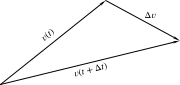
\includegraphics{figure/fig01.14}
 \caption{加速度的计算}
 \label{fig:01.14}
\end{wrapfigure}
一般如图\ref{fig:01.14}~所示。由于$a$平行于$\Delta v$,所以平均加速度的方向一
般与速度方向并不相同。瞬时加速度也类似。当加速度方向平行
于速度时,表示速度方向没有变化,但速率增加。当二者反平行
\clearpage\noindent
时,表示速度方向不变,而速率减少。当加速度既不平行也不反
平行于速度时,表示速度方向也在变化。

利用式\eqref{eqn:01.07.03},加速度矢量的分量可以表示为:
\begin{equation}\label{eqn:01.08.04}
 \vec{a}=\frac{\dif^2x\left(t\right)}{\dif t^2}\vec{i}+\frac{\dif^2y\left(t\right)}{\dif t^2}\vec{j}+\frac{\dif^2z\left(t\right)}{\dif t^2}\vec{k}
\end{equation}
加速度的三个坐标分量为:
\setlength{\mathindent}{4em}
\begin{equation}\label{eqn:01.08.05}
 a_x(t)=\frac{\dif^2x\left(t\right)}{\dif t^2},~ a_y(t)=\frac{\dif^2y\left(t\right)}{\dif t^2},~
 a_z(t)=\frac{\dif^2z\left(t\right)}{\dif t^2}
\end{equation}
\setlength{\mathindent}{6em}

$\vec{r}$,$\vec{v}$,$\vec{a}$是描写运动的物理量。我们希望用数目比较少的物
理量来描写运动。什么叫比较少?意思是这些物理量之间应是相
互独立的。所谓相互独立。是说其中任一个量不能由其他的量加
以确定。用$\vec{r}$,$\vec{v}$及$\vec{a}$三个量来描写运动是必要的,因为它们是相互
独立的。例如,在某一时刻,知道了质点的位置$\vec{r}$,并不能知道
它的速度$\vec{v}$,知道了$\vec{v}$,也并不能知道$\vec{a}$,反之亦然。人们认识到
这一点,也并不容易。在伽利略之前,并没有加速度概念。当时,
没有人认识到加速度与速度是相互独立的,所以没有认识到需要
用加速度来描写运动。

我们已讨论了位置矢量、速度和加建度。从运动学本身来考
虑,没有足够的理由说明,为什么我们应当到此为止,而不去讨
论加加速度、加加加速度……。当然,我们可以定义并计算加加
速度,即加速度的变化率,但一般说这并不代表任何具有基本物
理价值的东西。其中的原因在动力学,学过动力学后,我们将看
到,对力学的讨论几乎全部是基于位置矢量,速度和加速度这三
个量。

下面我们介绍运动的独立性这一重要概念。由式\eqref{eqn:01.05.02}、
\eqref{eqn:01.07.03}、\eqref{eqn:01.08.05}可以看到,描写一个复杂的曲线运动时,$X$方
向的坐标、速度、加速度与其他方向的坐标,速度、加速度无关。
$Y$方向和$Z$方向也有这种性质,即三个方向相互无关,这种性质被
称为运动的独立性。因此,一个复杂的曲线运动,可看成在$X$,$Y$,
$Z$三个方向上的直线运动,这三个运动同时进行,我们可以对每
一个运动进行单独的分析,好象另外两个自由度上的运动是根本
不存在一样,这样就使问题变得简单。

\example 已知一个质点作直线运动。观察到它的位置与时间
的变化如表\ref{tab:01.07}所示。用这些数据求出各时间间隔的平均速度$v$及
平均加速度$a$,并写出运动方程式。
\begin{table}[!h]
 \caption{}
 \label{tab:01.07}
 \centering
 \zihao{-5}
 \begin{tblr}{l*{9}{|X}}
 \toprule
 时~~~~间(秒) & 0 & 1 & 2 & 3 & 4 & 5 & 6 & 7 & 8 \\
 \midrule
 {与参考点的距离 (米)} & 3 & 4 & 9 & 18 & 31 & 48 & 69 & 94 & 123 \\
 \bottomrule
 \end{tblr}
\vspace{-0.8em}
\end{table}

\solution 因为时间间隔都是1秒,即$\Delta t=1$秒。所以从数值上有
\begin{align*}
 v & =\frac{\Delta s}{\Delta t}=\Delta s \\
 a & =\frac{\left(v_2-v_1\right)}{\Delta t}=v_2-v_1=\left(\Delta s_2\right)-\left(\Delta s_1\right)
\end{align*}
将结果列于表\ref{tab:01.08}中。
\begin{table}[!h]
 \caption{}
 \label{tab:01.08}
 \centering \zihao{-5}
 \setlength{\tabcolsep}{0em}
 \begin{tblr}{colsep=0pt,colspec={l*{17}{|X[c]}}}
 \toprule
 时~~~~间(秒) & 0 & & 1 & & 2 & & 3 & & 4 & & 5 & & 6 & & 7 & & 8 \\
 \midrule
 {与参考点的距离\\\qquad$s$~~(米)} & 3 & & 4 & & 9 & & 18 & & 31 & & 48 & & 69 & & 94 & & 123 \\
 {各秒内的位置变化\\\qquad$\Delta s$~~(米) } & & 1 & & 5 & & 9 & & 13 & & 17 & & 21 & & 25 & & 29 & \\
 {各秒内的平均速度\\\qquad$v$~~(米/秒)} & & 1 & & 5 & & 9 & & 13 & & 17 & & 21 & & 25 & & 29 & \\
 {各秒内的平均加速度\\\qquad$a$~~($\text{米/秒}^2$)} & & & 4 & & 4 & & 4 & & 4 & & 4 & & 4 & & 4 & & \\
 \bottomrule
 \end{tblr}
\end{table}
\clearpage
既然平均加速度$a$是一个常数,所以这个直线运动是匀加速
直线运动,加速度是$a=4$米/秒$^2$.对于匀加速直线运动,一般的
运动方程是:
%\vspace{-1em}
\begin{equation*}
 s=s_0+v_{0}t+\frac{1}{2}at^2 \vspace{-0.5em}
\end{equation*}
用已知数据代入,便可求出$s_0$,$v_0$,$a$。

当$t=0$时,$s=s_0=3$,所以$s_0=3$;

当$t=1$时,$4=3+v_0+\dfrac 1 2 a$,即$v_0+\dfrac 1 2 a=1$;

当$t=2$时,$9=3+2v_0+2a$,即$v_0+a=3$。

解上述两方程可得$a=4$,$v_0=-1$。所以运动方程式为:
\begin{equation*}
 s=3-t+2t^2
\end{equation*}

\example 在阴极射线管中,一束电子以$10^9$厘米/秒的速度水
平地射入平行板之间的均匀电场,电场使电子获得$10^{17}$厘米/秒\textsuperscript{2}
的向下的匀加速度。己知平行板长为2厘米。求:

\begin{wrapfigure}[8]{r}{16em}
 \centering
 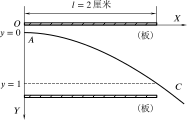
\includegraphics{figure/fig01.15}
 \caption{}
 \label{fig:01.15}
\end{wrapfigure}
(1)电子束通过平行板时的竖直方向位移$d$和经历
的时间$t$;

(2)电子束离开平行板时的速度大小和方向;

(3)在平行板内和离开板后电子束的轨迹。

\solution 选择如图\ref{fig:01.15}~所示的坐标系。

由于运动的独立性,在$x$方向是惯性运动,速度为$v_0=10^9$厘
米/秒;在$y$方向是匀加速运动,加速度为$a=10^{17}\text{厘米/秒}^2$(因为$a$
远远大于重力加速度$g$,所以不考虑重力的影响),且初速为零,
故有:

~\vspace{-1.5em}
\begin{equation*}
 \left\lbrace \begin{aligned}
 x & =v_0 t \\
 y & =\frac{1}{2}at^2+y_0
 \end{aligned}\right.
\end{equation*}
电子通过平行板的时间为:
\begin{equation*}
 t_0=\frac{l}{v_0}=\frac{2}{10^{9}}=\num{2e-9}\text{秒}
\end{equation*}
电子通过平行板时,在竖直方向的位移为:
\begin{align*}
 d & =y_1-y_0 \\
 & =\frac{1}{2}at_0^2 \\
 & =\frac{1}{2}\times 10^{17} \times \num{4e-18} \\
 & =0.2\text{厘米}
\end{align*}
电子在板中时,因为
\begin{equation*}
 v_x=v_0 \qquad v_y=at \\
\end{equation*}
\begin{align*}
 \beforetext{所以} v=\sqrt{v_x^2+v_y^2}=\sqrt{v_0^2 + a^2 t^2}
\end{align*}
速度与水平轴的夹角为:
\begin{equation*}
 \theta = \arctg\frac{v_y}{v_x} = \arctg\frac{at}{v_0}
\end{equation*}
它随时间而变。在离开板时,$t=t_0$,有
\begin{align*}
 & v \approx \num{1.02e9}\text{厘米/秒} \\
 & \theta = \arctg\frac{at_0}{v_0} =\arctg\frac 1 5=\ang{11;19;}
\end{align*}
在板内运动方程是:
\begin{equation*}
 \left\lbrace \begin{aligned}
 x & =v_0 t \\
 y & =\frac{1}{2}at^2+y_0
 \end{aligned}\right.
\end{equation*}
消去$t$则得$y=\dfrac{a}{2v_0^2}x^2+y_0$,轨迹是抛物线。

离开平行板后。电子以与水平轴成\,\ang{11;19;}\,的夹角的速度
$v\approx\num{1.02e8}$厘米/秒作直线运动。

\example 设在地面附近,重力加速度是个常数$g$,且垂直指向
地面。物体的初速度为$ v_0 $。与水平方向成$ \theta $角。试讨论抛体运动
轨迹。

\discussion 我们在$ v $和铅垂线所决定的平面上来研究。按图\ref{fig:01.16}~
中的坐标,可把运动分解为$ x $方向与$ y $方向,并分别处理。$ x $方向
是惯性运动$ v_x=v_0\cos\theta $,所以有
\begin{equation*}\label{xeqn:01.08.01}
 x=\left(v_0\cos\theta\right)t \tag{1}
\end{equation*}
$ y $方向就是上抛运动,初速度为$ v_0\sin\theta$。故有
\begin{align*}
 \label{xeqn:01.08.02} & v_y=v_0\sin\theta-gt \tag{2} \\
 \label{xeqn:01.08.03} & y=\left(v_0\sin\theta\right)t-\frac{1}{2}gt^2 \tag{3}
\end{align*}
由\eqref{xeqn:01.08.01},\eqref{xeqn:01.08.03}消去$ t $便得抛物线形的轨迹:
\begin{equation*}\label{xeqn:01.08.04}
 y=x \operatorname{tg} \theta-\frac{g x^{2}}{2 v_{0}^{2} \cos ^{2} \theta} \tag{4}
\end{equation*}
物体达到最高点时,$ v_y=0 $,由此便得在最高点处的时间为:
\begin{equation*}
 t_{1}=\frac{v_{0} \sin \theta}{g}
\end{equation*}
相应的最大高度为,
\begin{equation*}
 \begin{aligned}
 H & =v_{0} \sin \theta\left(\frac{v_{0} \sin \theta}{g}\right)-\frac{1}{2} g\left(\frac{v_{0} \sin \theta}{g}\right)^{2} \\
 & =\frac{v^{2} \sin ^{2} \theta}{2 g}
 \end{aligned}
\end{equation*}
物体落回到与出发点同样高度时,有:
\begin{equation*}
 y=0=v_{0} t \sin \theta-\frac{1}{2} g t^{2}
\end{equation*}
\clearpage
\begin{align*}
 \beforetext{即} t_{2}=\frac{2 v_{0} \sin \theta}{g}
\end{align*}
这时的水平距离$R$叫做射程:
\begin{equation*}
 R=\left(v_{0} \cos \theta\right) t_{2}=\frac{v_{0}^{2} \sin 2 \theta}{g}
\end{equation*}
\begin{wrapfigure}[7]{r}{16.5em}
 \centering
 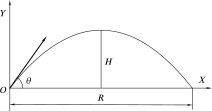
\includegraphics{figure/fig01.16}
 \caption{}
 \label{fig:01.16}
\end{wrapfigure}
因为当$\theta=\ang{45;;}$时,$\sin2\theta$
取最大值。所以,以同一速率$v_0$抛射物体,当
$\theta=\ang{45;;}$时,射程最远。
因为$\theta=\ang{90;;}$时,$\sin\theta$最
大,所以,只有当$\theta=\ang{90;;}$时,即竖直上抛,
$H$才能达到最大,其值为:
\begin{equation*}
 H_{\max }=\frac{v_{0}^{2}}{2 g}
\end{equation*}

这个题讨论的是理想情况,在实际情况中存在着空气阻力,
抛物速度愈大,阻力也愈大。空气阻力随着抛物速度的增加而逐
渐增加,在某一速度上将等于重力,这时物体将匀速下降。因而
实际上抛体的轨迹并不是理想的抛物线。

\section{圆周运动和角速度}\label{sec:01.09}

现在来讨论一种最简单的曲线运动——圆周运动。即轨迹是
个圆。如果选择圆心作为坐标原点,质点的位置就可用位置矢量
$\vec{r}$与某一选定的方向(例如$X$轴)之间的夹角$\varphi$(图\ref{fig:01.17})来描述,因
为$\varphi$确定之后,质点的位置就完全确定了。因而可用角$\varphi$与$t$的
关系$\varphi\left(t\right)$来代替函数$\vec{r}\left(t\right)$。

我们知道,对于直线运动,用一个坐标$x\left(t\right)$就可以描写。同
\clearpage
\noindent 样,对于圆周运动,也是只要一个坐标$\varphi\left(t\right)$来描写就够了。在这
\begin{wrapfigure}[9]{r}{13em}
  \centering \small
  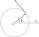
\includegraphics{figure/fig01.17}
  \caption{圆周运动}
  \label{fig:01.17}
\end{wrapfigure}
个意义上,两者是一样的。而一般的平面曲线运动,需要两个坐
标来描写;一般的空间曲线运动,则需要三个坐标来描写。我
们按描写运动所需坐标的个数,把运动分为一维运动、二维运动、
三维运动等等。直线运动和圆周运动都是一维运动。

按照\ref{sec:01.07}~节的讨论,速度的
方向为轨迹上相应点的切线方向,圆的切线总与半径相垂直,所
以圆周运动的速度$\vec{v}$总与位置矢量$\vec{r}$相垂直。现在来求速度的

\begin{wrapfigure}[8]{l}{13em}
  \vspace{-0.5em}
  \centering \small
  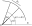
\includegraphics{figure/fig01.18}
  \caption{圆周运动的速率}
  \label{fig:01.18}
\end{wrapfigure}
\noindent 大小。由图\ref{fig:01.18},在$t$时刻,质点位于$\varphi\left(t\right)$;当$t+\Delta t$时,位于
$\varphi\left(t+\Delta t\right)$,所以在$\Delta t$间隔中质点
运动的路程为:
\setlength{\mathindent}{2em}
\begin{equation*}
  \begin{aligned}
    \Delta s & =r|\varphi\left(t+\Delta t\right)-\varphi\left(t\right)| \\
             & =r|\Delta \varphi|
  \end{aligned}
\end{equation*}
将此式代入式\eqref{eqn:01.07.05},就得到圆周运动的速率
\setlength{\mathindent}{6em}
\begin{equation}\label{eqn:01.09.01}
  v=\lim _{\Delta t \rightarrow 0} \frac{r|\Delta \varphi|}{\Delta t}=r \lim _{\Delta t \rightarrow 0} \frac{|\Delta \varphi|}{\Delta t}
\end{equation}
现在定义一个新的量,它是
\begin{equation}\label{eqn:01.09.02}
  \omega=\lim _{\Delta t \rightarrow 0} \frac{|\Delta \varphi|}{\Delta t}
\end{equation}
这种形式的公式我们已经多次遇到了。$|\Delta\varphi|/\Delta t$是在$t$到$t+\Delta t$间
隔中,质点的单位时间的角位置的平均变化。当取$\Delta t\rightarrow 0$的极限
时,这个平均变化率过渡为瞬时变化率。因此,我们称$\omega$为角速
度,确切地说,应称为角速率。它的单位是弧度/秒。利用角速率$\varphi$,式\eqref{eqn:01.09.01}可以写成
\begin{equation}\label{eqn:01.09.03}
  v=r\omega
\end{equation}

速度本质上是一个矢量,有大小和方向两方面。上述角速度
定义只反映了大小,为反映方向,我们需作些补充。

现在定义一个矢量$\vec{\omega}$,它的大小等于式\eqref{eqn:01.09.01}中的$\omega$,$ \vec{\omega}$的
方向按图\ref{fig:01.19}所示的方法给定。
\begin{figure}[!h]
  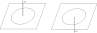
\includegraphics{figure/fig01.19}
  \caption{角速度的方向}
  \label{fig:01.19}
\end{figure}

\noindent 当我们从$ \vec{\omega}$指向的方向观察质点的运动时,质点总是沿逆时钟方
向转动。这个规定$ \vec{\omega}$的方向的方法也可以用一个正扣螺旋来说
明,当螺钉按质点运动方向旋转时,螺钉的运动方向就是$ \vec{\omega}$的方
向。

这样定义的$ \vec{\omega}$,称为角速度矢量。利用这个矢量。可以把质
点的速度矢量$\vec{v}$表示成
\begin{equation}\label{eqn:01.09.04}
  \vec{v}= \vec{\omega}\times \vec{r}
\end{equation}
由图\ref{fig:01.20},因为$ \vec{\omega}$与$\vec{r}$垂直,所以$| \vec{\omega}\times\vec{r}|=\omega r=v$,
而且$ \vec{\omega}\times\vec{r}$的方向与$\vec{v}$的方向一致。故式\eqref{eqn:01.09.04}
比\eqref{eqn:01.09.03}更具有一般性,它不仅表达了三者的大小关系,也反映了
三者间的方向关系。不仅如此,若取通过圆心且垂直于圆所在平面
的直线上任一点为原点(图\ref{fig:01.21})来描写圆周运动,式\eqref{eqn:01.09.04}仍成立,但式\eqref{eqn:01.09.03}就不对
\clearpage
\noindent 了。读者可以自己证明。

\begin{figure}[!h]
  \small
  \begin{minipage}[b]{15em}
    \centering
    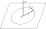
\includegraphics{figure/fig01.20}
    \vspace{4em}
    \caption{圆周运动中$ \vec{\omega}$与$\vec{v}$的关系}
    \label{fig:01.20}
  \end{minipage}
  \hfill
  \begin{minipage}[b]{13em}
    \centering
    \includegraphics{figure/fig01.21}
    \caption{原点不在圆心的情况}
    \label{fig:01.21}
  \end{minipage}
\end{figure}


\section{匀速圆周运动}\label{sec:01.10}

一般情况角速率$\omega$是随$t$变化的,这时质点的速度的大小也
随$t$变化。以下讨论$\omega$不随$t$变化的特殊情况,即匀速圆周运动。
由式\eqref{eqn:01.09.03},这时质点的速率也不变化。质点绕圆周一圈走过的
路程是$2\uppi r$。如果走一圈所用时间为$T$,则质点的速率是
\begin{equation}\label{eqn:01.10.01}
  v=\frac{2 \uppi r}{T}
\end{equation}
T为周期,比较式\eqref{eqn:01.10.01}、\eqref{eqn:01.09.03},得到:
\begin{equation}\label{eqn:01.10.02}
  \omega=\frac{2 \uppi}{T}, \quad T=\frac{2 \uppi}{\omega}
\end{equation}
这也就是说,周期$T$等于质点转过$2\uppi$角度所需要的时间。

对于匀速圆周运动,$\vec{v}$的大小不变,而$\vec{v}$的方向时时在变,因
而它的加速度并不为零。由于速度方向总是垂直于矢量$\vec{r}$的,所
以在$t$到$t+\Delta t$间隔中,倘使$\vec{r}$转过角度$\Delta\varphi$,
则$\vec{v}$也就转过了$\Delta\varphi$。由于
$|\vec{v}\left(t\right)|=|\vec{v}\left(t+\Delta t\right)|=v$,由图\ref{fig:01.22}~的等腰三角形,得
\begin{equation*}
  \begin{aligned}
    |\vec{v}\left(t+\Delta t\right)-\vec{v}\left(t\right)| & =2 v \sin \frac{\Delta \varphi}{2}                   \\
                                                           & \approx 2 v\frac{\Delta \varphi}{2}=v \Delta \varphi
  \end{aligned}
\end{equation*}

\begin{figure}[!h]
  \small\centering
  \begin{minipage}[b]{14em}
    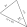
\includegraphics{figure/fig01.22}
    \vspace{1em}
    \caption{匀速圆周运动的加速度}
    \label{fig:01.22}
  \end{minipage}
  \begin{minipage}[b]{14em}
    \centering
    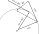
\includegraphics{figure/fig01.23}
    \caption{加速度的方向}
    \label{fig:01.23}
  \end{minipage}
\end{figure}
\noindent 将此式代入式\eqref{eqn:01.08.03},得
\begin{equation}\label{eqn:01.10.03}
  \begin{aligned}
    a & \equiv|\vec{a}|=\lim _{\Delta t \rightarrow 0} \frac{|\vec{v}\left(t+\Delta t\right)-\vec{v}\left(t\right)|}{\Delta t} \\
      & =v\lim_{\Delta t \rightarrow 0} \frac{|\Delta \varphi|}{\Delta t}=v \omega=r \omega^{2}=\frac{v^{2}}{r}
  \end{aligned}
\end{equation}\vspace{0.5em}
上式推导中利用了式\eqref{eqn:01.09.02},\eqref{eqn:01.09.03}。因为$v$或$\omega$都不随$t$变,
所以匀速圆周运动的加速度的大小也不随$t$变,但它的方向是时
时变化的。根据图\ref{fig:01.23},当$\Delta t\rightarrow 0$时,
$\vec{v}\left(t+ \Delta t\right)-\vec{v}\left(t\right)=\Delta\vec{v}$的方
向趋于与$\vec{v}\left(t\right)$相垂直,并指向圆心。这样,匀速圆周运动的加速
度的大小由式\eqref{eqn:01.10.03}给出,而其方向总是指向圆心的。根据这
种方向上的特点,称这个加速度为向心加速度。

速度、角速度和加速度都是矢量,我们可把式\eqref{eqn:01.10.03}扩充
为矢量关系式:
\clearpage
~\vspace{-1.56em}
\begin{equation}\label{eqn:01.10.04}
  \vec{a}= \vec{\omega}\times \vec{v}
\end{equation}
它的正确性也留给读者自己去证明。

\section{运动学里的反问题}\label{sec:01.11}

以上各节讨论的问题,都是当已知运动的轨迹函数$\vec{r}\left(t\right)$后,
求速度和加速度。在运动学中还会遇到一种相反的问题:已知质
点在各时刻的速度$\vec{v}\left(t\right)$,求它的轨迹函数$\vec{r}\left(t\right)$;已知加速度$\vec{a}\left(t\right)$,
求它的$\vec{v}\left(t\right)$。以前各节讨论的问题多与微分运算相联系,而这些
反问题,却是与积分运算相联系的。

仍然先讨论直线运动。如果已知直线运动的质点的速度为
$v\left(t\right)$,并已知在$t=0$时,质点在$x\left(0\right)$(称为初始位置),求在时刻
t的质点的坐标$x\left(t\right)$。

我们把零到$t$这段时间间隔,分成许多小段,即$\Delta t_1 , \Delta t_2 , \cdots$,
而且$\Delta t_1+\Delta t_2+\cdots=t$,如果所有各小段都相当小,则在每个间隔
中速度变化不太大,在$\Delta t_i$中速度近似为$v\left(t_i\right)$。这样,在每个时
间间隔中质点的坐标变化分别近似为:
\begin{equation*}
  \begin{array}{l}
    \Delta x_{1} \approx v\left(t_{1}\right) \Delta t_{1} \\[-1pt]
    \Delta x_{2} \approx v\left(t_{2}\right) \Delta t_{2} \\[-1pt]
    \cdots \cdots
  \end{array}
\end{equation*}
因而,质点在0到$t$间隔中坐标的总变化$x\left(t\right)-x\left(0\right)$就应当等于
这许多小变化的总和,即\vspace{-0.5em}
\begin{equation}\label{eqn:01.11.01}
  \begin{aligned}
    x\left(t\right)-x\left(0\right) & =\Delta x_{1}+\Delta x_{2}+\Delta x_{3}+\cdots    \\[-1pt]
                                    & \approx \sumx_{i} v\left(t_{i}\right) \Delta t_{i}
  \end{aligned}
\end{equation}
各时间间隔$\Delta t_i$取得越小,计算结果就越准确,当所有$\Delta t_i\rightarrow 0$时,
就得到质点位置变化的精确值:

~\vspace{-1.56em}
\begin{equation}\label{eqn:01.11.02}
  x\left(t\right)=x\left(0\right)+\lim _{\Delta t_{i} \rightarrow 0} \sumx_{i} v\left(t_{i}\right) \Delta t_{i}
\end{equation}
上式取极限的项,与积分的定义是一样的。所以它可写成
\begin{equation}\label{eqn:01.11.03}
  x\left(t\right)=x\left(0\right)+\int_{0}^{t} v\left(t\right) {~\mathrm d}  t
\end{equation}
这就是我们所要求的答案。

现在说明式\eqref{eqn:01.11.01}或\eqref{eqn:01.11.02}中求和运算的几何意义。我
们在图\ref{fig:01.24}~中画出了速度$v$对时间$t$的关系曲线。各时间间隔$\Delta t_1 , \Delta t_2 , \cdots$,相应于横坐标上的各小段,各$v\left(t_1\right) , v\left(t_2\right) , \cdots$,相应
于各小段中$ v $的近似值。因而$\Delta x_1 , \Delta x_2 , \cdots$,在数值上就等于相
应的小长方形的面积。故对所有$\Delta x_i$求和,在各小段$\Delta x_i$都趋于
无限小的情况下,在数值上就等于零到$t$间横轴之上与曲线$v$之
下所围的面积。

利用这种几何性质,对一些简单情况,计算式\eqref{eqn:01.11.03}中的
积分是很容易的。下面举两个例子。
\begin{figurex}[!h]
  \begin{minipage}[b]{14em}
    \centering
    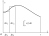
\includegraphics[width=0.8\linewidth]{figure/fig01.24}
    \caption{运动的$v-t$图}
    \label{fig:01.24}
  \end{minipage}\hfill
  \begin{minipage}[b]{14em}
    \centering
    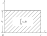
\includegraphics[width=0.8\linewidth]{figure/fig01.25}
    \caption{匀速运动的$v-t$图}
    \label{fig:01.25}
  \end{minipage}
\end{figurex}

\example 匀速运动。

如果质点的速度是常数$v_0$,它的$v-t$图就如图\ref{fig:01.25}~所示。由0
到$t$的横轴与曲线$v$围成一个长方形,它的面积是$v_0t$,将之代入
式\eqref{eqn:01.11.03},即得轨迹函数为:
\begin{equation}\label{eqn:01.11.04}
  x\left(t\right)=x\left(0\right)+v_0 t
\end{equation}
~\vspace{-1.5em}
\begin{figure}[!h]
  \begin{minipage}[b]{14em}
    \centering
    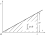
\includegraphics[width=0.8\linewidth]{figure/fig01.26}
    \caption{匀加速运动的$v \mathdash t$图}
    \label{fig:01.26}
  \end{minipage}\hfill
  \begin{minipage}[b]{14em}
    \centering
    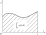
\includegraphics[width=0.8\linewidth]{figure/fig01.27}
    \caption{运动的$a-t$图}
    \label{fig:01.27}
  \end{minipage}
\end{figure}

\vspace{-1em}\example 匀加速运动。

设质点的速度与时间成正比,$v=at$,在图\ref{fig:01.26}~中画出这个
关系。零到$t$的横轴与曲线$v$围成一个直角三角形,它的面积是
$\dfrac{1}{2} a t^2$,代入式\eqref{eqn:01.11.03},就得到轨迹函数为:
\begin{equation*}\label{eqn:01.11.04i}
  x\left(t\right)=x\left(0\right)+\frac{1}{2}at^2 \tag{1.11.4$'$}
\end{equation*}

已知加速度$a\left(t\right)$,求速度$v\left(t\right)$的方法,同样可以按上面的方
法求得,将0到$t$的时间间隔分成小段$\Delta t_1 , \Delta t_2 , \cdots$,每个小段中
加速度分别近似为$a\left(t_1\right) , a\left(t_2\right) , \cdots$,因而在每个小段中,速度的
变化相应为$\Delta v_1\approx a\left(t_1\right)\Delta t_1 , \Delta v_2\approx a\left(t_2\right)\Delta t_2 , \cdots$,在0到$t$间隔中速
度总的变化等于所有变化之和,即
\begin{equation}\label{eqn:01.11.05}
  \begin{aligned}
    v\left(t\right)-v\left(0\right) & =\Delta v_{1}+\Delta v_{2}+\cdots                 \\
                                    & \approx \sumx_{i} a\left(t_{i}\right) \Delta t_{i}
  \end{aligned}
\end{equation}
其中$v\left(0\right)$是$t=0$时质点的速度,称为初速度。
同样,取所有$\Delta t _ i \to 0$的极限,就得到速度变化的精确表达式为,
\begin{equation}\label{eqn:01.11.06}
  \begin{aligned}
    v\left(t\right) & =v\left(0\right)+\lim _{\Delta t_{i} \rightarrow 0} \sumx _ i a\left(t_{i}\right) \Delta t_{i} \\
                    & =v\left(0\right)+\int_{0}^{t} a\left(t\right) {~\mathrm d}  t
  \end{aligned}
\end{equation}
上式中积分的几何意义是$a-t$图中由0到$t$的横轴与$a$曲线之间
所围的面积(图\ref{fig:01.27})。

对于曲线运动的情况,式\eqref{eqn:01.11.03}、\eqref{eqn:01.11.06}分别推广成
{\setlength{\mathindent}{4em}
%\setlength\abovedisplayskip{0pt}
%\setlength\belowdisplayskip{0pt}
\setlength{\lineskip}{-1pt}
\setlength{\lineskiplimit}{-1pt}
\begin{eqnarray}
  \label{eqn:01.11.07}
  \begin{aligned}
    \vec{r}\left(t\right)= & \vec{r}\left(0\right)+\int_{0}^{t} \vec{v}\left(t\right) {~\mathrm d}  t \\
    =                      & \vec{r}\left(0\right)
    +\left(\int_{0}^{t} v_{x}\left(t\right) {~\mathrm d}  t\right) \vec{i}
    +\left(\int_{0}^{t} v_{y}\left(t\right) {~\mathrm d}  t\right) \vec{j}                            \\
                           & +\left(\int_{0}^{t} v_{z}\left(t\right) {~\mathrm d}  t\right) \vec{k}
  \end{aligned} \\
  \label{eqn:01.11.08}
  \begin{aligned}
    \vec{v}\left(t\right)= & \vec{v}\left(0\right)+\int_{0}^{t} \vec{a}\left(t\right) {~\mathrm d}  t \\
    =                      & \vec{v}\left(0\right)
    +\left(\int_{0}^{t} a_{x}\left(t\right) {~\mathrm d}  t\right) \vec{i}
    +\left(\int_{0}^{t} a_{y}\left(t\right) {~\mathrm d}  t\right) \vec{j}                            \\
                           & +\left(\int_{0}^{t} a_{z}\left(t\right) {~\mathrm d}  t\right) \vec{k}
  \end{aligned}
\end{eqnarray}
\setlength{\mathindent}{6em}}%
其中$\vec{r}\left(0\right)$及$\vec{v}\left(0\right)$分别为初始时刻质点的位置矢量及速度矢量。具
体使用式\eqref{eqn:01.11.07}及\eqref{eqn:01.11.08}时,可以把它们分解成分量的关系
来计算。式\eqref{eqn:01.11.07}等价于下列三式。
{%\setlength\abovedisplayskip{0pt}
%\setlength\belowdisplayskip{0pt}
\setlength{\lineskip}{-1pt}
\setlength{\lineskiplimit}{-1pt}
\begin{equation}
  \begin{aligned}\label{eqn:01.11.09}
    x\left(t\right)=x\left(0\right)+\int_{0}^{t} v_{x}\left(t\right) {~\mathrm d}  t \\
    y\left(t\right)=y\left(0\right)+\int_{0}^{t} v_{y}\left(t\right) {~\mathrm d}  t \\
    z\left(t\right)=z\left(0\right)+\int_{0}^{t} v_{z}\left(t\right) {~\mathrm d}  t
  \end{aligned}
\end{equation}}%
而式\eqref{eqn:01.11.08}等价于下列三式。
{\setlength\abovedisplayskip{0pt}
\setlength\belowdisplayskip{0pt}
\setlength{\lineskip}{-1pt}
\setlength{\lineskiplimit}{-1pt}
\begin{equation}\label{eqn:01.11.10}
  \begin{aligned}
    v_x\left(t\right)=v_x\left(0\right)+\int_{0}^{t} a_{x}\left(t\right) {~\mathrm d}  t \\
    v_y\left(t\right)=v_y\left(0\right)+\int_{0}^{t} a_{y}\left(t\right) {~\mathrm d}  t \\
    v_z\left(t\right)=v_z\left(0\right)+\int_{0}^{t} a_{z}\left(t\right) {~\mathrm d}  t
  \end{aligned}
\end{equation}}%
这些积分中没有出现矢量,就可以按一一般方法计算,譬如上述的
面积方法就是一种可行的方法.

研究运动有两种次序。一种是先研究轨迹,已知轨迹函数为
$\vec{r}\left(t\right)$,再来推求速度$\vec{v}\left(t\right)$,加速度$\vec{a}\left(t\right)$。就人类的认识过程来说,的
确是先看到轨迹的形状,然后有了运动快慢的概念,最后认识到
速度的变化,即加速度。另一种次序是:先知道加速度,然后再
求速度及轨迹。在物理学中,从力学的规律来看。往往是如此。

前一种次序,看上去非常自然,是人类研究机械运动所走的
一条路。在牛顿之前,亚里士多德认为轨迹是最基本的,速度则
次之。这种方法的特点是先研究运动的大的整体方面,然后再涉
及局部细节。

后一种次序,是牛顿创建的方法。也是现代物理学一个基本
的方法。牛顿认为,不要先探讨物体运动的整体方面。而是先研
究运动的瞬时情况,瞬时情况更为基本。弄清瞬时情况之后再来
讨论整体运动。也可以说,这种方法是先研究局部细节,然后再
作积分,得到整体性质。至今在大多数情况下,物理学家仍采取
牛顿的这种方法。

上述两种方法反映了两种不同的信念。一种认为整体的大的
方面更简单些,因此,主张从大到小的研究顺序;另一种认为局
部的单元过程更简单些,因此。主张从小到大的研究顺序。我们
将在第五章说明,这两种“简单性”可能是分不开的。
\begin{questions}

  \question 一个原则上不能进行直接或间接测量的物理量是否有意
  义?

  \question 平均速率有两种意思,一是指平均速度矢量的大小,一
  是指物体运动路径总长度除以所用的总时间。这两种意思是否相
  同?

  \question 质点作一维运动,如果加速度不是恒量,质点的平均速率
  是否等于$\dfrac 1 2$(初速+末速)?

  \question 当物体的加速度恒定不变时,它的运动方向可否改变?

  \question 质点的运动方程为$x=x\left(t\right)$,$y=y\left(t\right)$。在计算它的速度和
  加速度的大小时,有人先求出$r=\sqrt{x^2+y^2}$,然后根据$v=\dfrac{ \dif r}{ \dif t}$,
  $a=\dfrac{ \dif ^2r}{ \dif t^2}$,求得结果;有人先计算速度和加速度分量,再合成,所
  得结果为:\vspace{-1em}
  \begin{equation*}
    \begin{aligned}
      v & =\sqrt{\left(\frac{ \dif  x}{ \dif  t}\right)^{2}+\left(\frac{ \dif  y}{ \dif  t}\right)^{2}}                 \\
      a & =\sqrt{\left(\frac{ \dif ^{2} x}{ \dif  t^{2}}\right)^{2}+\left(\frac{ \dif ^{2} y}{ \dif  t^{2}}\right)^{2}}
    \end{aligned}
  \end{equation*}
  你认为哪一组结果正确?

  \question  两千多年前,住在尼罗河口亚历山大城的埃拉托色尼,首
  估算出地球的半径。然而,真正沿着地球子午线用绳长及日晷对
  地球进行测量的,却是中国唐代高僧一行(公元683$\sim$727)。你知
  道高僧一行测量的原理,方法及计算结果吗?

  \question  设想将一小球上抛。如不考虑空气阻力,试证明它返回原
  地时的速率等于开始的速率,并证明上升和下落所经过的时间相
  等。

  \question  将一小球铅直地上抛,若考虑空气阻力,它上升和下降所
  经过的时间哪一个长?

  \question  假设有两石块$m$和$M$,其中$m$较轻,$M$较重。按照亚里士多
  德的看法,在地面上$M$应该比$m$下落得快些。伽利略首先用思辨
  的方式指出亚里士多德的看法是自相矛盾的。伽利略说,设想将
  $m$与$M$系在一起,则构成物体$\left(m+M\right)$,此物下落时,因为$m$有下
  落得较慢的趋势,所以,$m$应该阻碍$M$,使它下落得比$m$快些而又
  比$M$慢些;但是另一方面,物体$\left(m+M\right)$比$M$还要重,按照亚里
  士多德的看法,它应比$M$下落得更快。因此,导致矛盾。

  你认为伽利略的推理是否正确?

  \question  质点在空间的运动,一般是三维运动。忽略风的作用的抛
  体运动,为什么可以作为二维运动来处理?
\end{questions}

\begin{exercises}

\exercise 用芝诺时计算阿基里斯的速度$v_1'$和加速度$a_1'$,并给出$x \mathdash t'$图。

\exercise 甲乙两列火车在同一水平直路上以相等的速率(30公里/时)
相向而行。当它们相隔60公里的时候,一只鸟以60公里/时的
恒定速率离开甲车头向乙车头飞去,一当到达立即返回,如此来
回往返不止。试求:

(1)当两车头相遇时,鸟往返了多少次?

(2)鸟共飞行了多少时间及距离?

(3)我们定义一种特殊的“小鸟钟”:小鸟从一车头到另一车
头为小鸟钟的时间测量单位(即小鸟钟的一个“滴答”)。用小鸟
钟记时的数值为$t''$求$t''$与一般时钟记时$t$之间的变换。

\exercise 一人从$O$点出发,向正东走3.0米,又向正北走1.0米,
\begin{wrapfigure}[8]{r}{8.5em}
  \begin{center}
    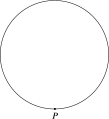
\includegraphics{figure/fig01.28}
    \caption{}
    \label{fig:01.28}
  \end{center}
\end{wrapfigure}
然后向东北走2.0米,试求合位移的大小及方向。

\exercise 一质点从$ P $出发,向左以匀速率1.0厘米/秒沿半径为$R=1.0$米的圆周运动(图\ref{fig:01.28})。问:

(1)当它走过2/3圆周时,位移是多少?走过的路程是多少?在这段时间内的
平均速度是多少?该点的瞬时速度是多少?

\clearpage
(2)当它走过1/2圆周时,以上各值又如何?

\exercise 一物体作直线运动,它的位置由方程$x=10t^2+6$决定,其
中$x$的单位为厘米,$t$的单位为秒,试计算:

(1)在$ 3.00\sim 3.10 $秒、$ 3.000\sim 3.01 $秒及$ 3.000\sim 3.001 $秒间
隔内的平均速度;

(2)在$t=3.00$秒时的瞬时速度;

(3)用微分方法求它的速度及加速度公式。

\exercise 有一质点沿x方向作直线运动,t时刻的坐标为:
\begin{equation*}
  x=4.5t^2-2t^3
\end{equation*}
式中$x$的单位为米。$t$的单位为秒。试求:

(1)第2秒内的位移和平均速度;

(2)第1秒末和第2秒末的瞬时速度;

(3)第2秒内质点所走过路径的长度;

(4)第2秒内的平均加速度以及第0.5秒末和第1秒末的瞬时
加速度。

\exercise 一质点以恒定的径向速度$r=4$米/秒在一平面中运动。它
的角速度为常量,其大小为$\omega=\dot\theta=2$弧度/秒。当质点距原点为3
米时,它的速度的大小及加速度大小是多少?

\exercise 如图\ref{fig:01.29}所示,向上抛一物体,测量物体上抛及下落经
\begin{wrapfigure}[10]{r}{13em}
  \begin{center}
    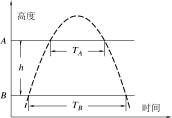
\includegraphics{figure/fig01.29}
    \caption{}
    \label{fig:01.29}
  \end{center}
\end{wrapfigure}
过水平线$A$的时差$T_A$,以及上抛
及下落经过水平线$B$的时差$T_B$。
试证明,若忽略空气阻力,重力
加速度的大小可以表示为:
\begingroup
\setlength{\mathindent}{4em}
\begin{equation*}
  g=\dfrac{8h}{T_A^2 - T_B^2}
\end{equation*}
\endgroup
式中$h$是$B$线与$A$线的高度差。

\exercise 天体物理常涉及大尺度的
问题,为了方便起见,引进一些
实用的大的长度单位。一个天文单位(AU)等于从地球到太阳的
平均距离;一个秒差距是一个天文单位所张之角为1秒的距离,即
观测者从某一恒星看地球公转轨道半径所张的角度为1秒时,该恒
星与太阳之间的距离。试求。

(1) 1秒差距相当于多少米?多少天文单位?及多少光年?

(2)以秒差距为单位,表示地球到太阳的距离。

\exercise 一物体从离地面的高度为$ h $的地方,由静止开始自由下
落,经过最后196米所用的时间是4.0秒钟。求物体下落过程所用
的总时间及其高度。

\exercise 一枚从地面发射的火箭以20米/$\text{秒}^2$的匀加速度竖直上升
半分钟后,燃料用完,于是象一个自由质点一样运动。略去空气
阻力,试求。

(1)火箭达到的最大高度;

(2)它从离开地面到再回地面所经过的总时间。

\exercise 把两个小物体从同一地点以同样初速率$v_0=24.5$米/秒
先后竖直上抛,设抛出两物体的时差为$\Delta t=0.500$秒,试问:

(1)第二个物体抛出后,经过多少时间$t$才与第一个物体相遇?

\vspace{-0.15em}(2)如果$\Delta t\geqslant\dfrac{2v_0}{g}$,讨论结果的物理意义。\vspace{-0.15em}

\exercise 物体以初速$v_0=20$米/秒被抛出,抛射仰角是\ang{60;;},略去
空气阻力,试问:

(1)物体开始运动后的1.5秒末,运动方向与水平方向的夹角
$\alpha$是多少?2.5秒末夹角$\alpha$又为多少?

(2)物体抛出后经过多少时间,运动方向才与水平成\ang{45;;}角?
这时物体的高度是多少?

(3)在物体轨迹最高点处的曲率半径$R_1$有多大?

(4)在物体落地点处,轨迹的曲率半径$R_2$有多大?

\exercise 高台下降滑雪在一平滑的山坡上进行。山坡与水平线成
恒定角度$\alpha$,滑雪运动员初速率为$v_0$,并以与水平线成$\theta$的仰角跳
出(\ref{fig:01.30})。若不考虑空气阻力,试证明:
\begin{figure}[h]
  \centering
  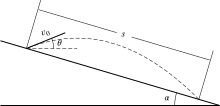
\includegraphics{figure/fig01.30}
  \caption{}
  \label{fig:01.30}
\end{figure}

(1)运动员落在斜坡上的距离为:
\begin{equation*}
  s=\frac{2 v_{0}^{2} \sin \left(\theta+\alpha\right) \cos \theta}{g \cos ^{2} \alpha}
\end{equation*}

(2)对于一定的$v_0$和$\alpha$来说,$s$在$\theta=\ang{45;;}-\dfrac{\alpha}{2}$时有最大值。其
值为:
\begin{equation*}
  s_{\max }=\frac{v_{0}^{2}\left(1+\sin \alpha\right)}{g \cos ^{2} \alpha}
\end{equation*}

\exercise 1977年中国男子铁饼的最好记录是54.28米,1983年提高
到60米。这些记录都是在北京创造的,北京的重力加速度$g$为
980.12厘米/$\text{秒}^2$。设投掷点比落地点高1.5米,略去空气阻力,
问投掷时至少要用多大的初速度,才可达到上述距离?

\exercise 设若干个光滑斜面($a_1, a_2, a_3, \dots $)有共同的底边$b$为30
厘米。试问:

(1)斜面与水平夹角$\alpha$为多大时,才能使物体在该斜面上从顶
端自由滑至底上正好需时为$t=0.4$秒?

(2)多大的夹角$\alpha$,使下滑的时间最短?

\exercise 在空间某一点$O$以相同的速率向各方向同时把若干小
球搬出去。试证明在略去空气阻力的情况下,任一时刻$t$,所有小
球都位于一个球面上,并求:

(1)此球心的运动方程式;

(2)球面距球心的距离。

\exercise 若抛射体的初速率为$v_0$,抛射角为$\theta$,略去空气阻力。伽
利略说:“抛射角为$\ang{45;;}+\delta$和$\ang{45;;}-\delta\left(\delta<\ang{45;;}\right)$的两个抛射体初速
率相同时,射程是相等的。”试证明他的话,并证明$\theta=\ang{45;;}$时水
平射程最大。

\begin{wrapfigure}[8]{r}{13em}
  \vspace{-2.5em}
  \begin{center}
    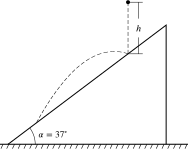
\includegraphics{figure/fig01.31}
    \caption{}
    \label{fig:01.31}
  \end{center}
\end{wrapfigure}
\exercise 一弹性球自由下落在一斜面上,与斜面发生完全弹性碰
撞,下落高度$h=20$厘米,斜面对水平的倾角$\alpha=\ang{37;;}$(图\ref{fig:01.31})。若
不计空气阻力,它第二次碰到斜面的位置距原来的下落点多远?

\exercise 用枪瞄准空中的靶,当子弹射出枪口时,靶同时自由下
落。如果略去空气阻力。不论子弹速率多大,总会击中下落的靶,
这个现象叫做百发百中,说明其中理由。

\exercise 一轰炸机高海面10公里,以240公里/小时的水平速度追
击正前方一鱼雷艇,鱼雷艇的速度是95公里/小时,不计空气阻
力,问飞机应在艇后多少距离投弹才能正好击中目标?

\exercise 一俯冲轰炸机沿与铅垂线成$\ang{37;;}$方向俯冲,在800米高度
投弹,炸弹离开飞机5.0秒钟时着地。不计空气阻力,试问:

(1)飞机的飞行速度是多少?

(2)炸弹离开飞机后在水平方向前进多远?

(3)炸弹着地时,速度的大小和方向?

\exercise 应以多大的水平速度$v$把一物体从高$h$处抛出,才能使
它在水平方向的射程为$h$的$n$倍?

\exercise 飞机以360公里/小时的速度由东向西飞行。试回答:

(1)在什么地理纬度上,飞机上的人可以看见太阳不动地停
在空中?

(2)若在极地附近沿纬线以圆轨道由东向西飞行,可以看见
什么现象?

\exercise 一俯冲轰炸机以不变的速率450公里/小时俯冲后。急离
俯冲线改为沿一铅垂平面内的圆形路线飞行。试问:要使飞机在
圆的最低点的加速度不超过$7g$,圆形路线的最小半径应是多少?

\exercise 车轮在地平面上作匀角速的纯滚动,轮行的速度为$v_0=
  10$米/秒,轮的半径为$r=0.50$米,试求;

(1)车轮边缘上一点$A$的角速度$\omega$;

(2)$A$点的轨迹。

\exercise 一半径为$r$的小球沿两固定的等高平行导轨作纯滚动,
两导轨间的距离为$d$,如图\ref{fig:01.32}所示。试问:

(1)球心的速度与球的角速度的关系是怎样的?

(2)小球面上一点$A$的轨迹如何?
\begin{figure}[h]
  %\vspace{-1em}
  \begin{center}
    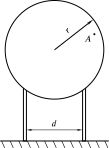
\includegraphics{figure/fig01.32}
    \caption{}
    \label{fig:01.32}
  \end{center}
\end{figure}

\end{exercises}

